%!TEX root=../main.tex
\section{Results} % (fold)
\label{sec:results}

\subsection{Decomposition of the densities} % (fold)
\label{sub:decomposition_of_the_densities}

We apply MFPCA to estimate the mean functions and eigenfunctions, providing a description of player shooting behavior. Figure~\ref{fig:mean_eigenfunctions} presents the estimation of the mean functions alongside the estimated functional principal components, which capture deviations from the mean shooting density. Unlike the shooting densities, the functional principal components may take on negative values as they represent deviations from the mean rather than densities themselves. For presentation purposes, the functional principal components have been normalized between $-1$ and $1$. Blue areas correspond to negative values of the functional components, and thus contribute negatively to the density, while red area corresponds to positive values of the functional components, and thus contribute positively to the density. The mean chart represents the shooting behavior of the average player in the NBA. Shots are most frequently taken in the paint, then the most common position is behind the three-point line, in the wings and the corners. We remark that the elbows and the short-corners are less important as shooting spots. The estimated functional components can be explained as characterising different shooting behaviors. We first note that, except for $\phi_3$, the functional components for missed and made shots are similar. This suggests  that players do not have specific shooting position where the percentage of missed shots significantly exceeds that of made shots. The first component, explained $67.9\%$ of the total variance, contrasts players based on their overall shooting frequency relative to the average NBA player. A player with a positive score $c_1$ for $\phi_1$ will shots more frequently, both successfully and unsuccessfully, than average. These effects are mainly focused on the high-density areas of the court such as the paint and beyond the arc (i.e., $\phi_1$ has a similar shape to the mean function). Conversely, a negative score corresponds to players who shoot less frequently than the average, with effects concentrated in these same regions. The second component (explaining $8.5\%$ of the total variance) highlights a contrast between shooting inside and outside the three-pointer line. Players with a positive score $c_2$ for $\phi_2$ prefer to shoot closer to the basket, while those with negative scores prefer long-range shots. The third component (explaining $6.1\%$ of the total variance) contrasts players that shoot in the paint and the others. Positive scores $c_3$ are associated with frequent attempts and successes in the paint, while negative scores would prefer to shoot farther out. Interestingly, players who perform well near the basket also tend to attempt and miss shots from the corners. The fourth component (explaining $4.0\%$ of the total variance) captures differences between shooting from the wings and shooting along the axis of the hoop. Players with positive (resp. negative) score will shot in the axis of the hoop (resp. from the wing). 
\begin{figure}
    \centering
    
\includegraphics[scale=0.35]{figures/mean.eps}
    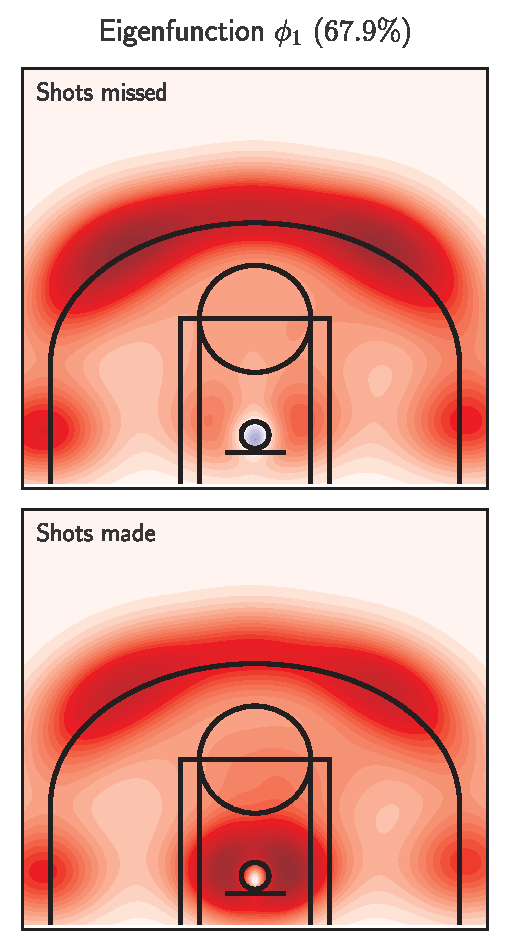
\includegraphics[scale=0.35]{figures/eigenfunction_1.eps}
    
\includegraphics[scale=0.35]{figures/eigenfunction_2.eps}
    
\includegraphics[scale=0.35]{figures/eigenfunction_3.eps}
    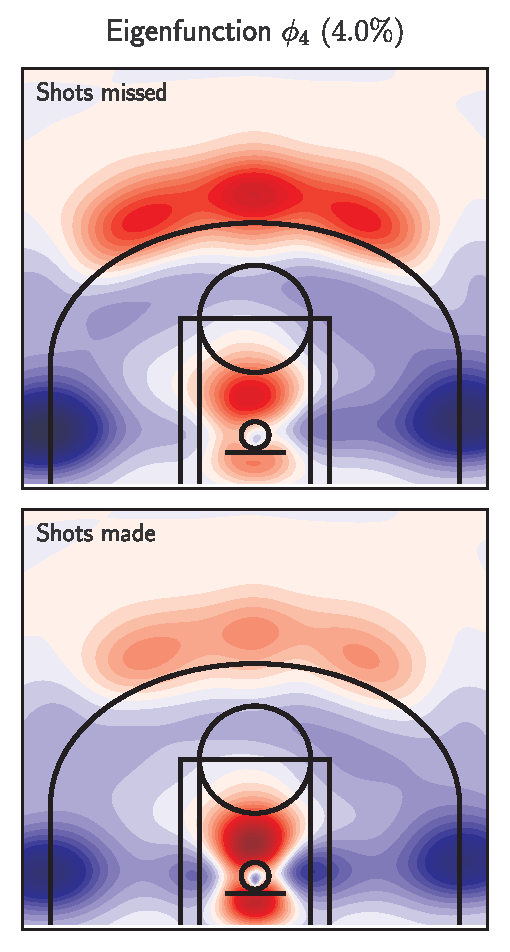
\includegraphics[scale=0.35]{figures/eigenfunction_4.eps}
    \\
    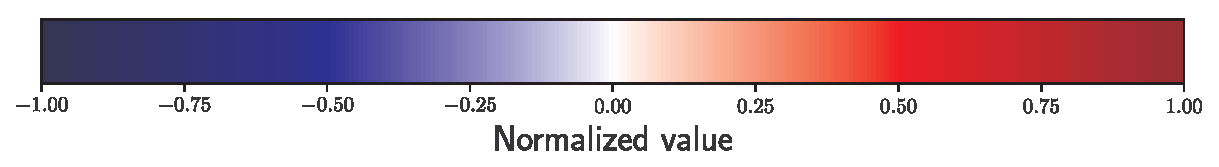
\includegraphics[scale=0.35]{figures/colorbar2.eps}
    \caption{Estimation of the mean surface and the eigenfunctions of the density shots charts. The eigenfunctions represent deviation from the mean surface and are defined up to a sign. Their values at specific points are thus not interpretable \emph{per se}. Note that the mean surface and eigenfunctions have been normalized between $-1$ and $1$ for presentation purpose.}
    \label{fig:mean_eigenfunctions}
\end{figure}

As an example, Figure~\ref{fig:examples_players} presents the decomposition of Stephen Curry. We remark that he shots more than the average player, because he miss and make more shots that the average player, as his first coefficient $c_1$ is positive. He does have a little preference for shooting behind the three-points line as his second coefficient is close to $0$. Its coefficient $c_3$ is a small negative values, indicating that he is around average for this eigenfunction. However, he prefers to shoots in the axis of the basket (positive coefficient $c_4$) compare to the other players. 
\begin{figure}
    \centering
    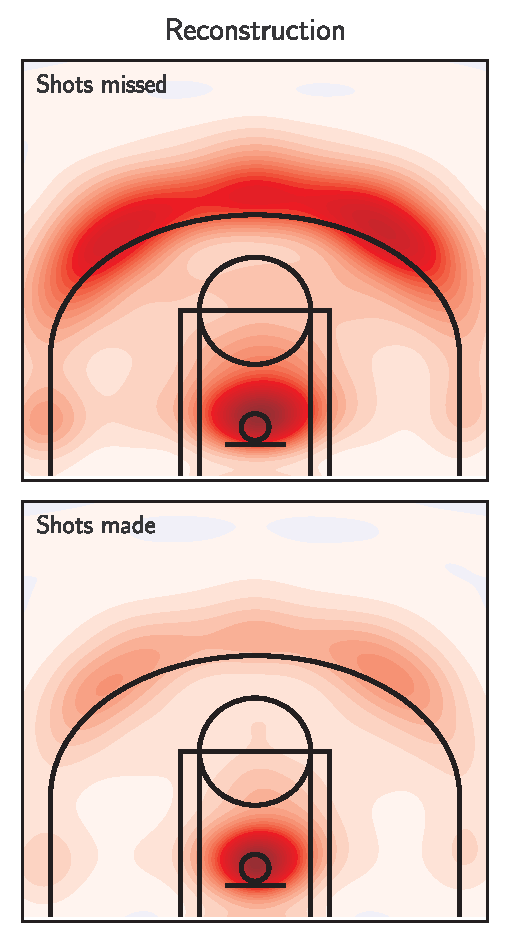
\includegraphics[scale=0.295]{figures/curry_reconstruction.eps}
    
\includegraphics[scale=0.295]{figures/mean.eps}
    
\includegraphics[scale=0.295]{figures/curry_eigenfunction_1.eps}
    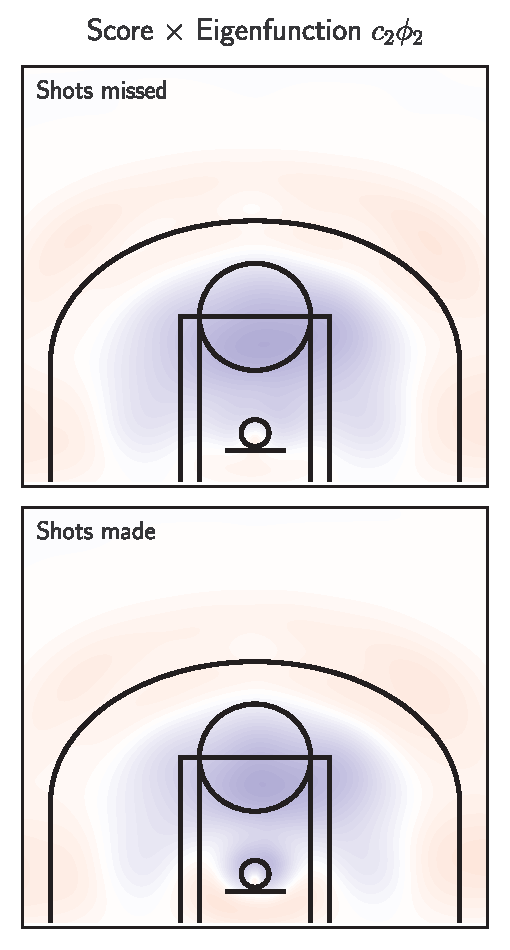
\includegraphics[scale=0.295]{figures/curry_eigenfunction_2.eps}
    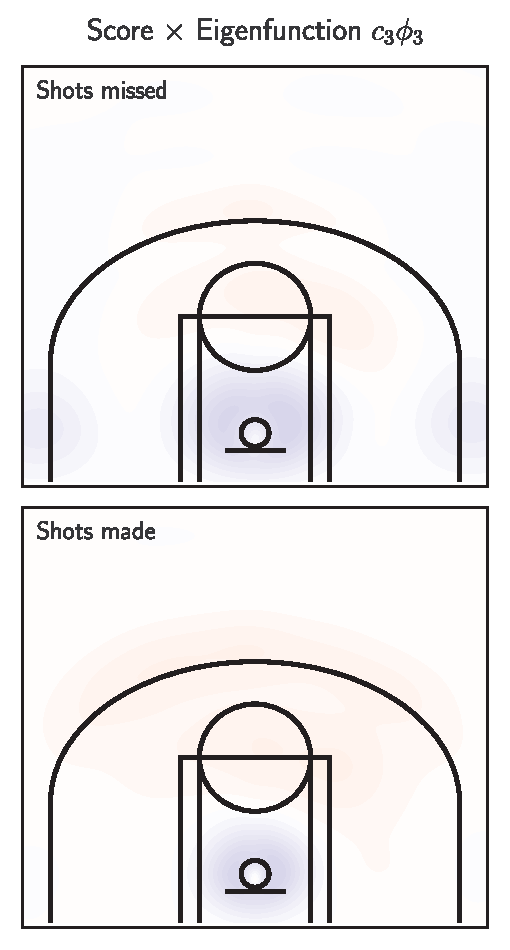
\includegraphics[scale=0.295]{figures/curry_eigenfunction_3.eps}
    
\includegraphics[scale=0.295]{figures/curry_eigenfunction_4.eps}
    \\
    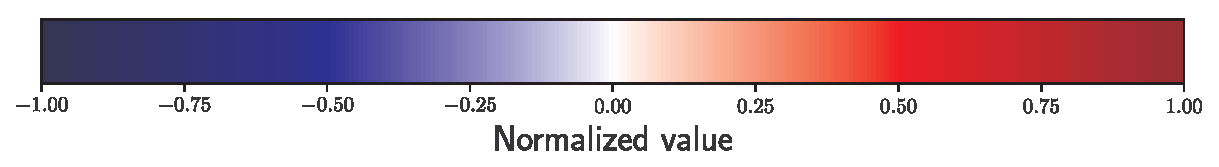
\includegraphics[scale=0.35]{figures/colorbar2.eps}
    \caption{Example of the decomposition of Stephen Curry into the eigenfunctions basis.}
    \label{fig:examples_players}
\end{figure}

Figure~\ref{fig:clusters} presents the estimated scores $c_k$ from~\eqref{eq:kl_decomp} colored by their playing position according to the NBA. We highlight the scores of one player per position. We remark that no score can distinguish the players typology as defined by the NBA as the scores of each position are overlapping one another. From Figure~\ref{fig:clusters}, we remark that some players exhibit scores (coefficients) that are very different than the other players. For example, for the second eigenfunction, Chris Paul (with a large coefficient) and Duncan Robinson (with a large negative coefficient) may be designed as outliers. Similarly, for the third eigenfunction, Chris Paul has a large negative coefficient. It may seems contradictory for Chris Paul, as a positive $c_2$ is explained as a preference for shooting from the painted area and a negative $c_3$ is explained as a preference for shooting from the three-points line. However, this is explained by the fact that the most common shooting position of Chris Paul is the high post (between the three-point line and the painted area), and so the eigenfunctions are compensating each others. This situation is not common in today's NBA. Finally, for the fourth eigenfunction, Reggie Bullock Jr. has a large negative coefficient, indicating a large preference for shooting from the wings and corners.
\begin{figure}
    \centering
    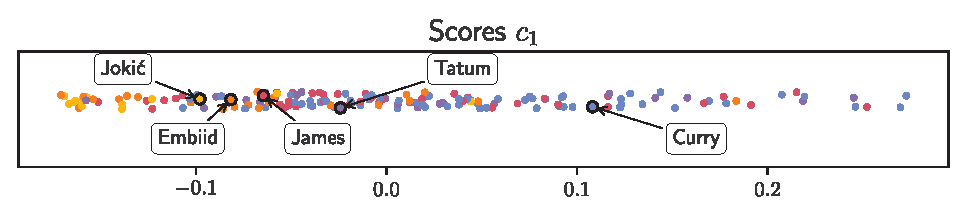
\includegraphics[scale=0.95]{figures/scores_1.eps}
    
\includegraphics[scale=0.95]{figures/scores_2.eps}
    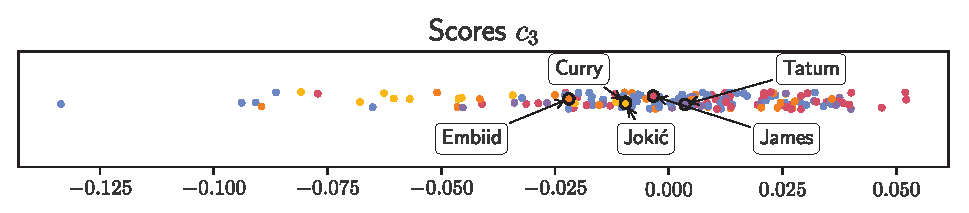
\includegraphics[scale=0.95]{figures/scores_3.eps}
    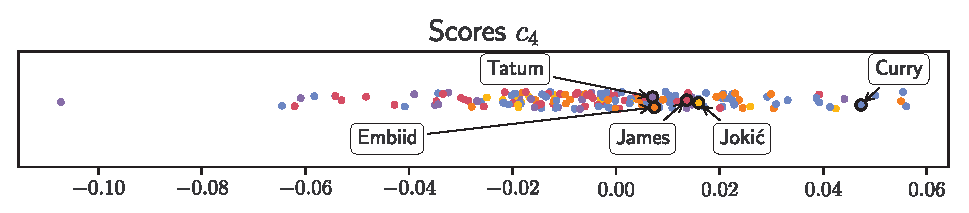
\includegraphics[scale=0.95]{figures/scores_4.eps}
    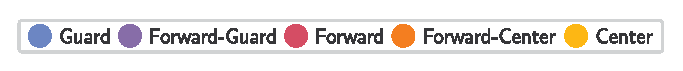
\includegraphics[scale=0.95]{figures/legend.eps}
    \caption{Scatter plots of the coefficients colored using the NBA defined typology of players. We highlighted one player per position. The scores have been jittered on the y-axis for visualisation purposes.}
    \label{fig:clusters}
\end{figure}


% subsection decomposition_of_the_densities (end)

\subsection{Clustering} % (fold)
\label{sub:clustering}

The $k$-medoids algorithm has been applied to the coefficients plotted in Figure~\ref{fig:clusters} as described in Section~\ref{sec:method}. We are aiming for $5$ clusters as the number of players on the court for each team. The complete clustering results are given the Appendix~\ref{sec:clustering_results}. To explain the clusters, we compute the mean coefficients per cluster and multiply by the eigenfunctions. It results in the decomposition of the average player within each cluster. The decompositions differ noticeably between the clusters. Figures~\ref{fig:average_cluster_no_weight} and~\ref{fig:average_cluster_weight} represent the decomposition for the average player of each cluster. For the interpretation of each cluster, we recall that the decomposition must be interpreted with respect to an average player, and the eigenfunctions represent a deviation from the mean. 


\begin{figure}
    \centering
    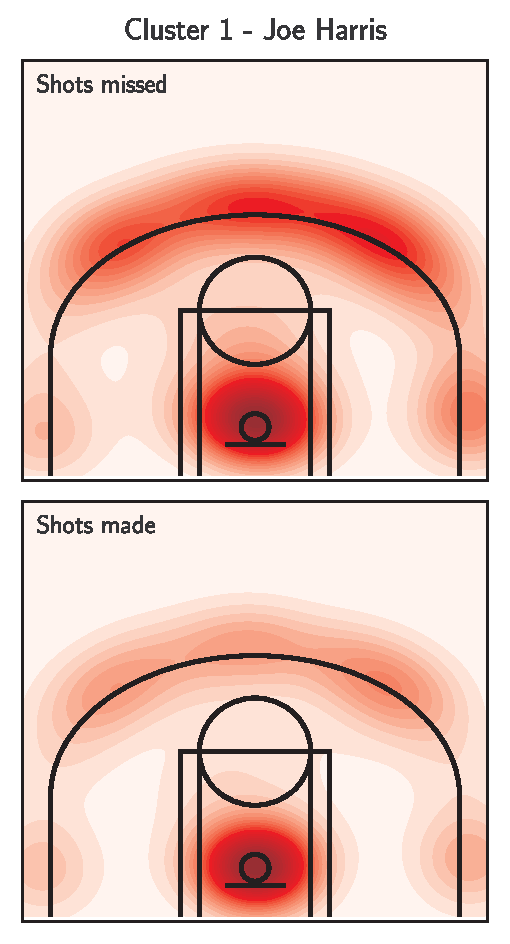
\includegraphics[scale=0.35]{figures/average_player_1.eps}
    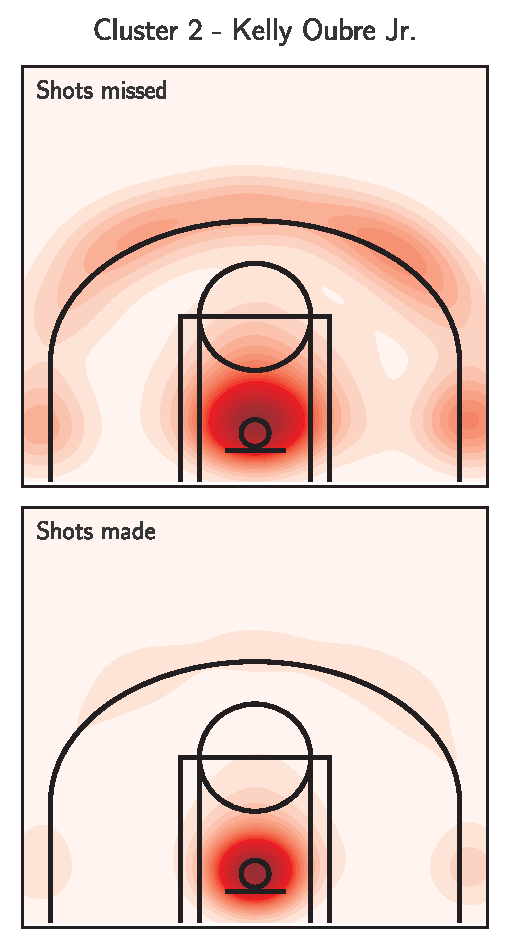
\includegraphics[scale=0.35]{figures/average_player_2.eps}
    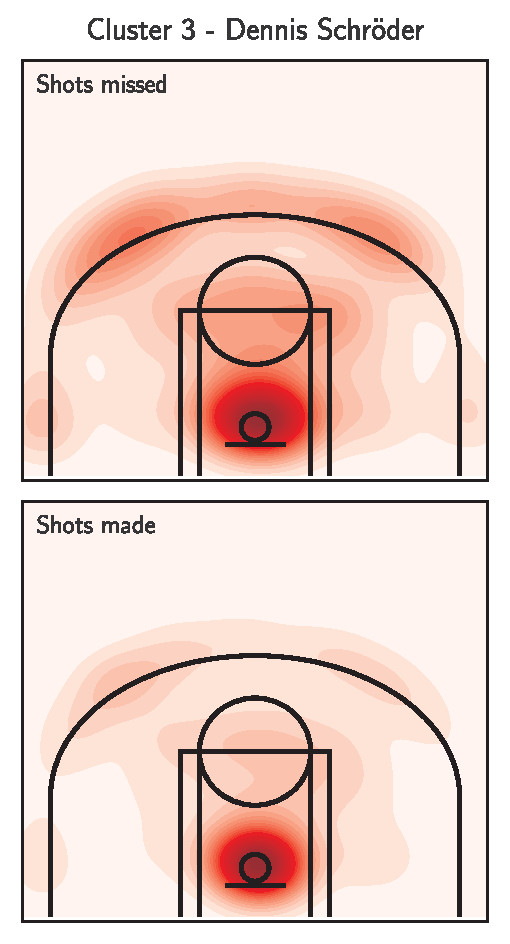
\includegraphics[scale=0.35]{figures/average_player_3.eps}
    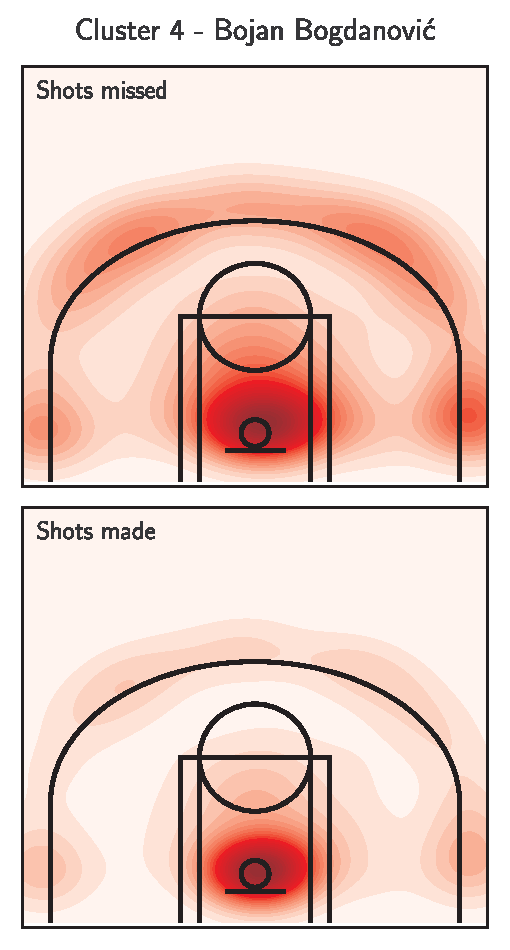
\includegraphics[scale=0.35]{figures/average_player_4.eps}
    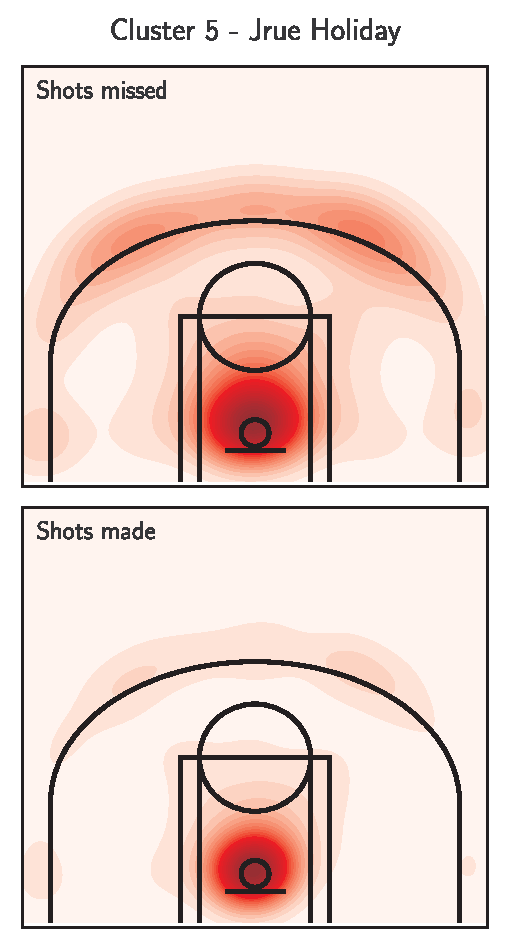
\includegraphics[scale=0.35]{figures/average_player_5.eps}
    \caption{Most representative player of each cluster.}
    \label{fig:average_cluster_no_weight}
\end{figure}

\begin{figure}
    \centering
    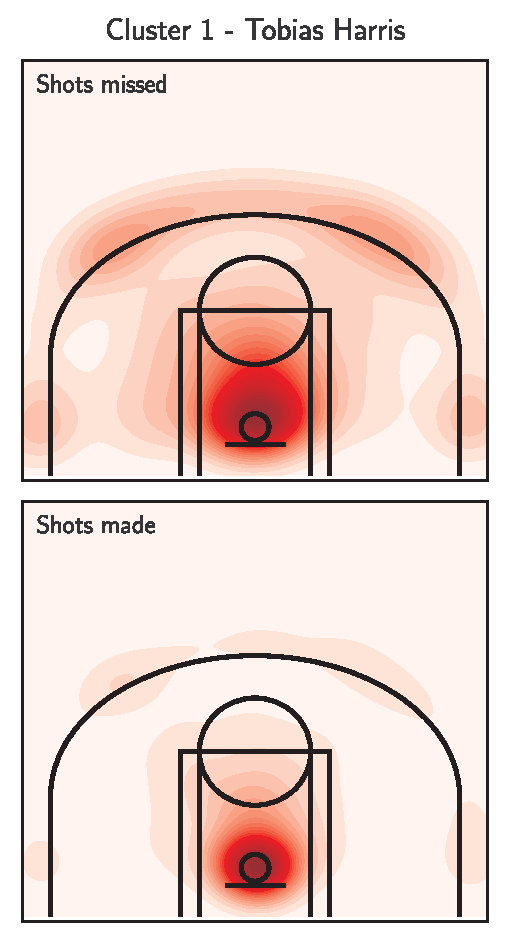
\includegraphics[scale=0.35]{figures/average_player_1_weighted.eps}
    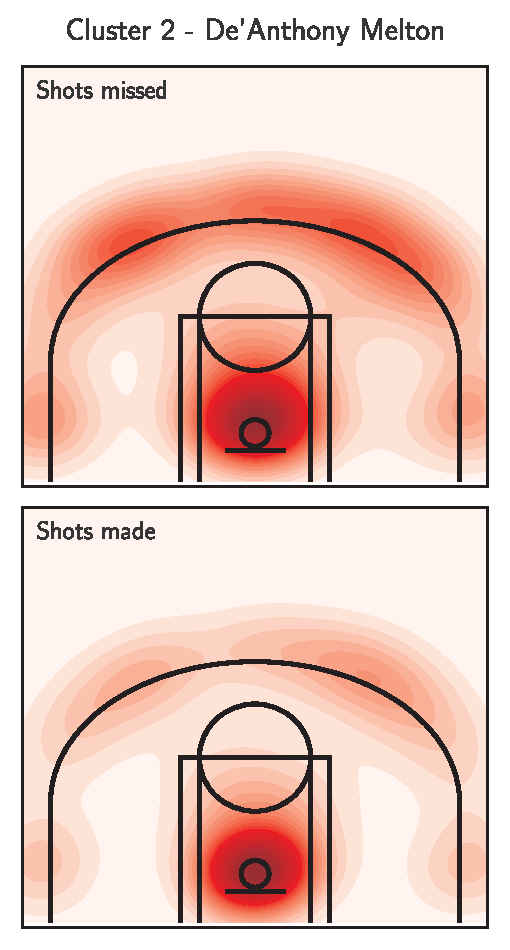
\includegraphics[scale=0.35]{figures/average_player_2_weighted.eps}
    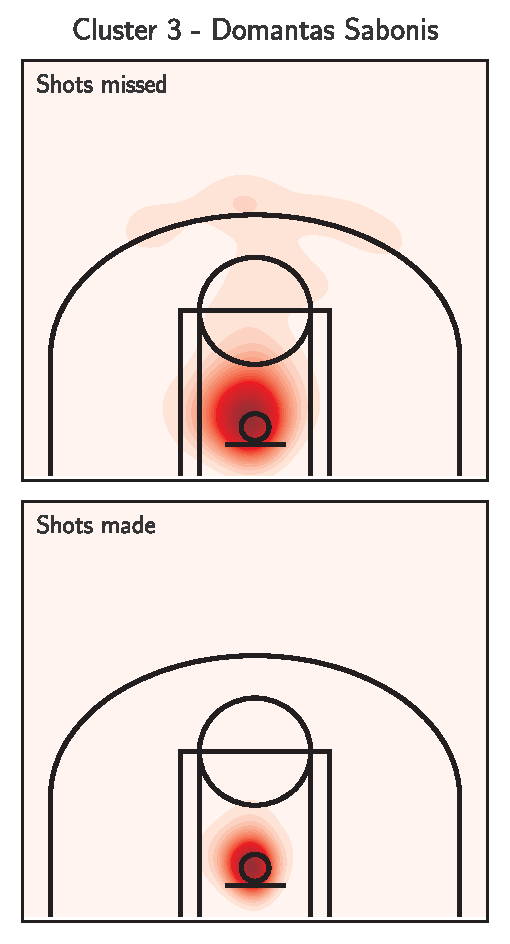
\includegraphics[scale=0.35]{figures/average_player_3_weighted.eps}
    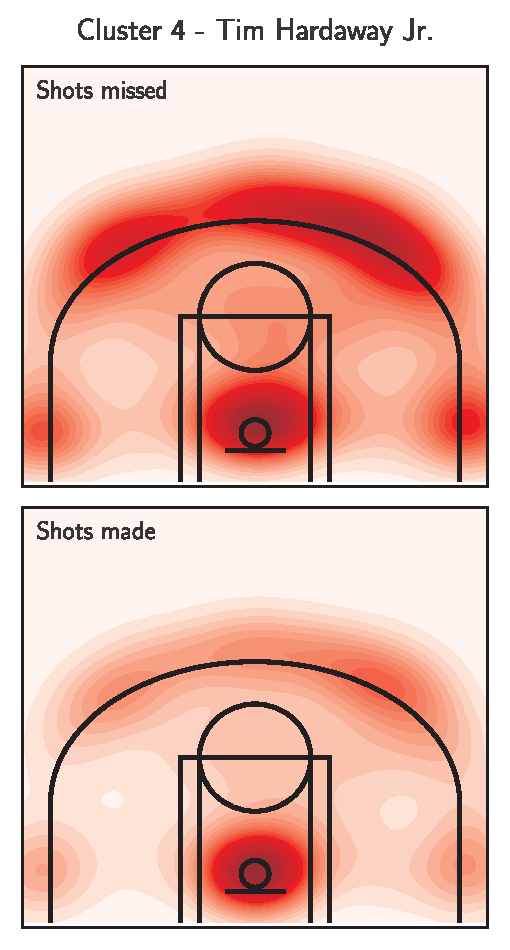
\includegraphics[scale=0.35]{figures/average_player_4_weighted.eps}
    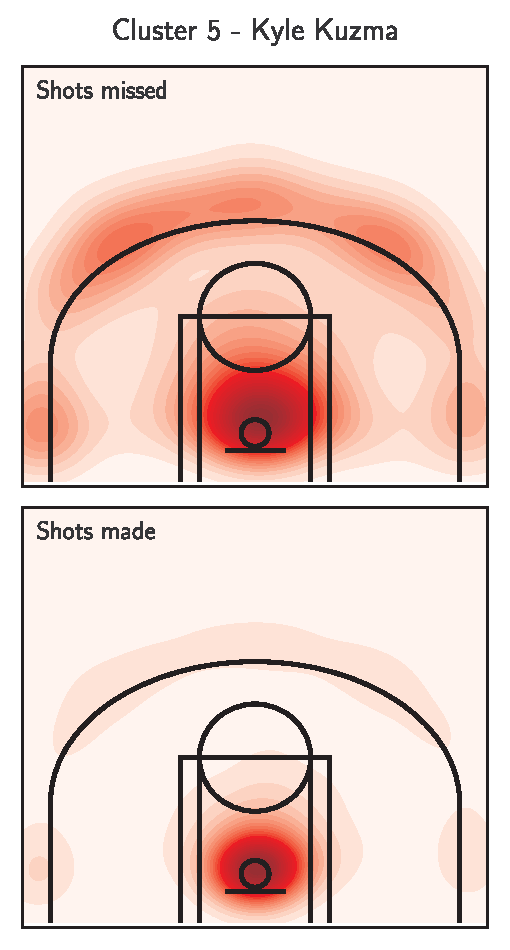
\includegraphics[scale=0.35]{figures/average_player_5_weighted.eps}
    \caption{Most representative player of each cluster.}
    \label{fig:average_cluster_weight}
\end{figure}


\begin{figure}
    \centering
    \begin{subfigure}{0.32\textwidth}
        \centering
        
\includegraphics[scale=0.5]{figures/confusion_mat_kmedoids_no_weights.eps}
        \caption{NBA / No weights.}
    \end{subfigure}
    \hfill
    \begin{subfigure}{0.32\textwidth}
        \centering
        
\includegraphics[scale=0.5]{figures/confusion_mat_kmedoids_weights.eps}
        \caption{NBA / Weights.}
    \end{subfigure}
    \hfill
    \begin{subfigure}{0.32\textwidth}
        \centering
        
\includegraphics[scale=0.5]{figures/confusion_matk_medoids_w_no_w.eps}
        \caption{Weights / No weights}
    \end{subfigure}
    \caption{Confusion matrices.}
    \label{fig:confusion_mat}
\end{figure}




% \begin{table}
% \centering
% \caption{Example of players in each clusters}
% \label{tab:example_players_clusters}
% \begin{tabular}{ cccccc } 
%  Cluster 1 & Cluster 2 & Cluster 3 & Cluster 4 & Cluster 5 \\ 
%  \hline
%  B. Adebayo & S. Curry & D. Boker & J. Crowder &  L. James \\
%  G. Antetokounmpo & E. Fournier & L. Dončić & J. Holiday & N. Jokić \\
%  B. Simmons & K. Love & J. Harden & P. Mills & J. Tatum \\
%  R. Gobert & K. Lowry & K. Irving & D. Robinson & K.-A. Towns \\
%  M. Robinson & C. Paul & K. Leonard & L. Shamet & J. Embiid \\
% \end{tabular}
% \end{table}

% From Figure~\ref{fig:clusters_1}, the average player in cluster $1$ tend to shot less than the other players (coefficient from the first eigenfunction is negative).
% \begin{figure}
%     \centering
%     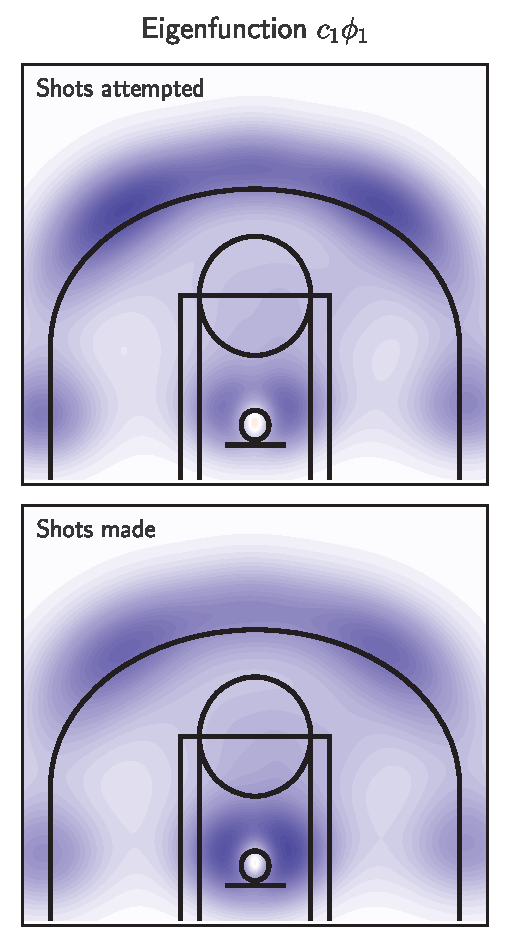
\includegraphics[scale=0.4]{figures/cluster_1_eigenfunction_1.eps}
%     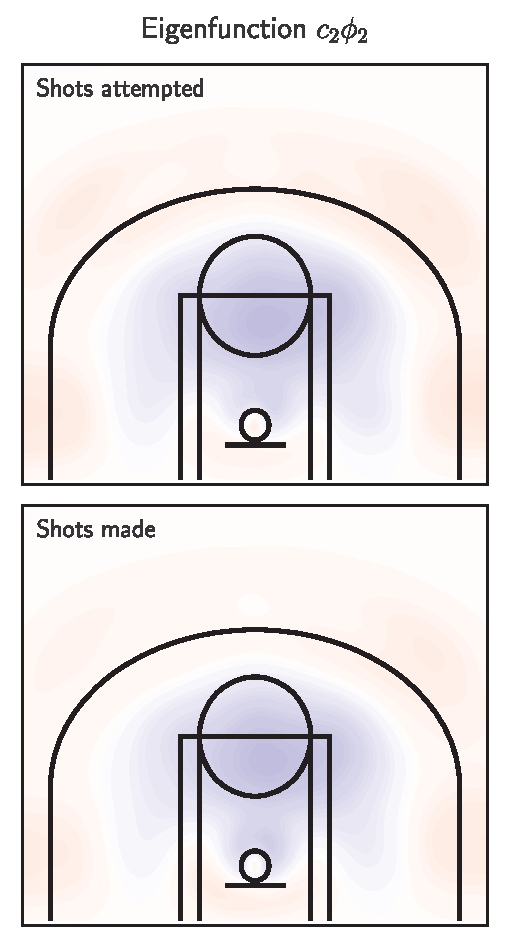
\includegraphics[scale=0.4]{figures/cluster_1_eigenfunction_2.eps}
%     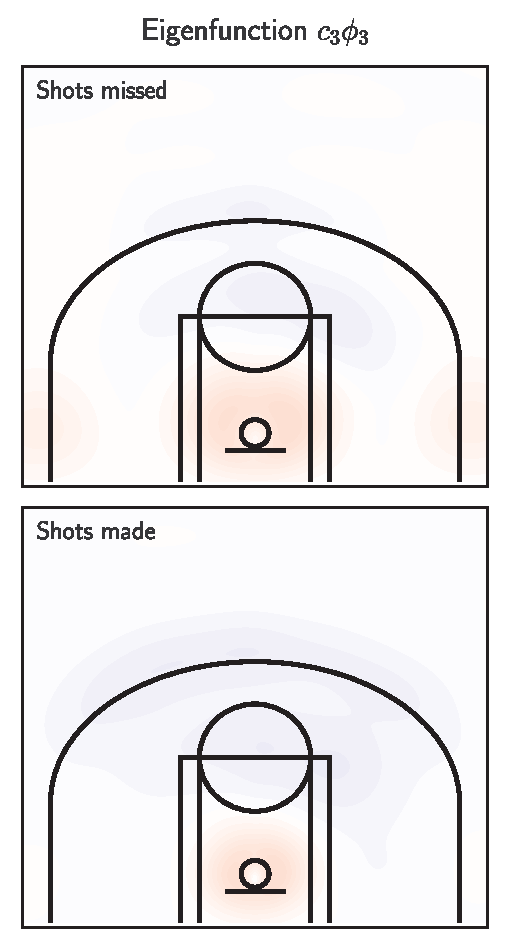
\includegraphics[scale=0.4]{figures/cluster_1_eigenfunction_3.eps}
%     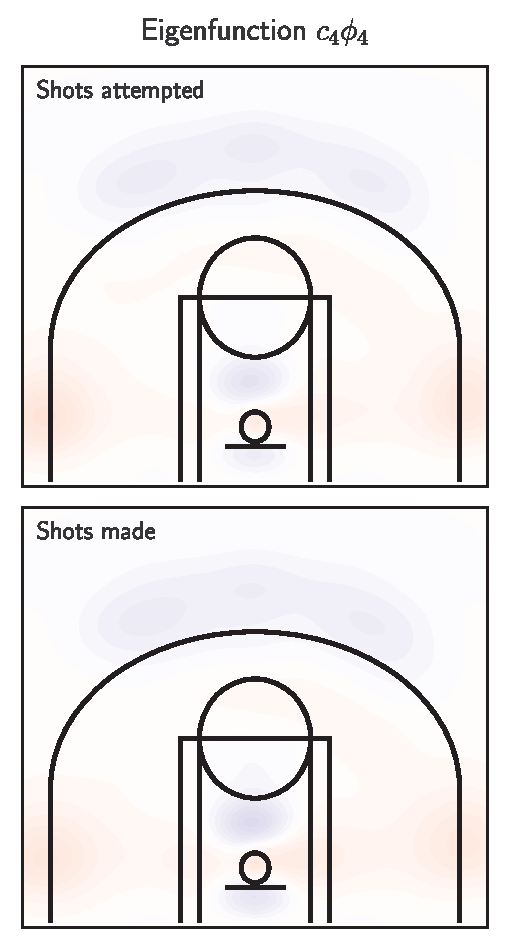
\includegraphics[scale=0.4]{figures/cluster_1_eigenfunction_4.eps}
%     \caption{Cluster 1}
%     \label{fig:clusters_1}
% \end{figure}

% From Figure~\ref{fig:clusters_2}, the average player in cluster $2$ tend to shot more than the other players (coefficient from the first eigenfunction is positive). These players do not have shooting preference as the coefficients of the second to fourth eigenfunctions is close to $0$.
% \begin{figure}
%     \centering
%     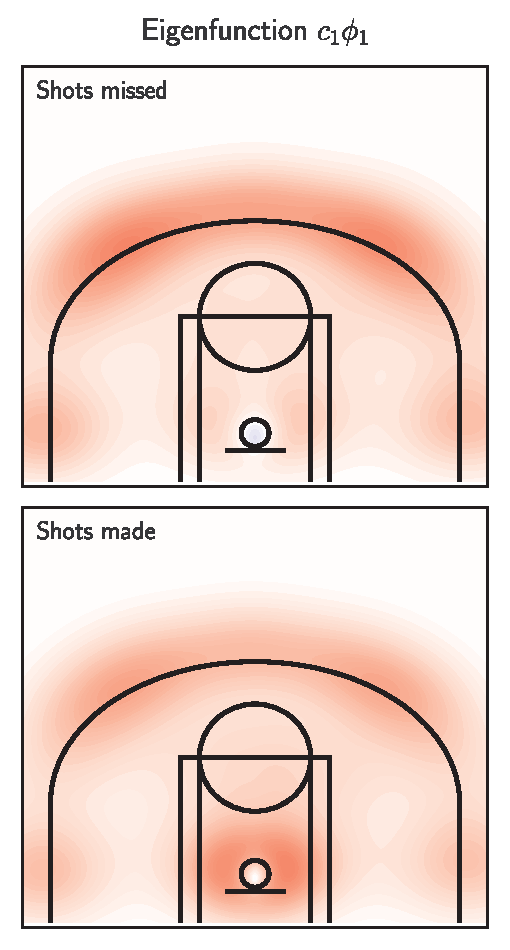
\includegraphics[scale=0.4]{figures/cluster_2_eigenfunction_1.eps}
%     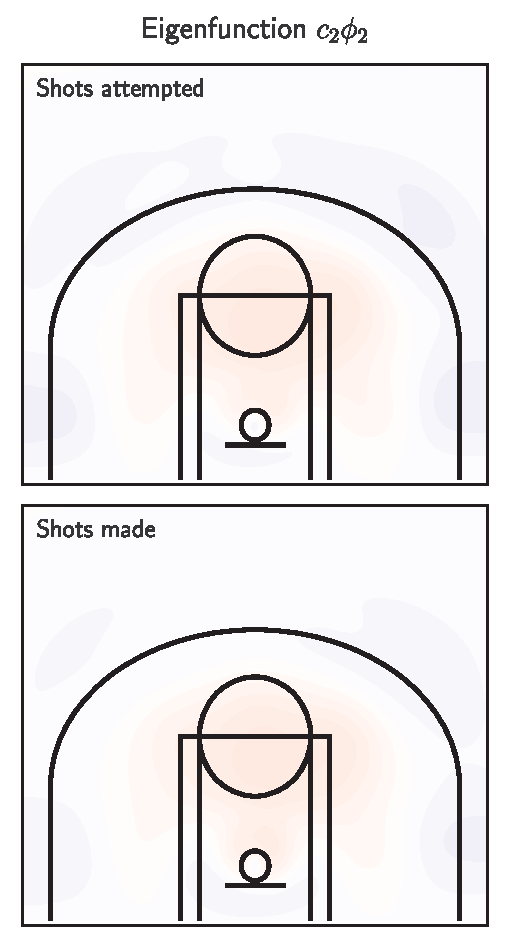
\includegraphics[scale=0.4]{figures/cluster_2_eigenfunction_2.eps}
%     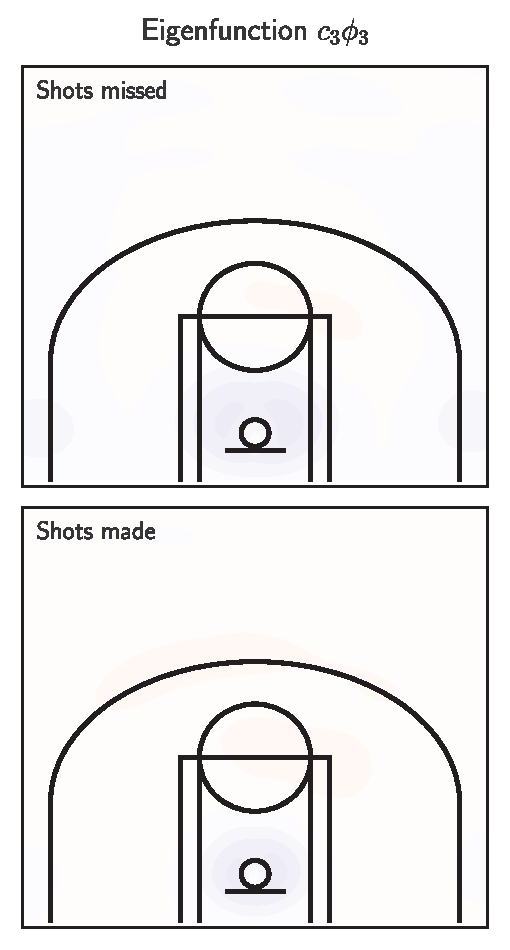
\includegraphics[scale=0.4]{figures/cluster_2_eigenfunction_3.eps}
%     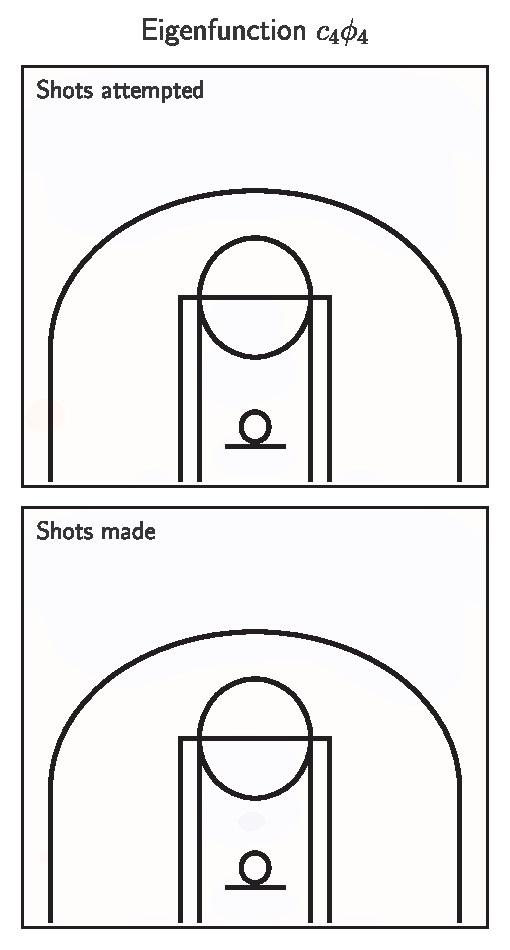
\includegraphics[scale=0.4]{figures/cluster_2_eigenfunction_4.eps}
%     \caption{Cluster 2}
%     \label{fig:clusters_2}
% \end{figure}

% From Figure~\ref{fig:clusters_3}, players in cluster $3$ are average players in the NBA. Their coefficients for each eigenfunction is close to $0$.
% \begin{figure}
%     \centering
%     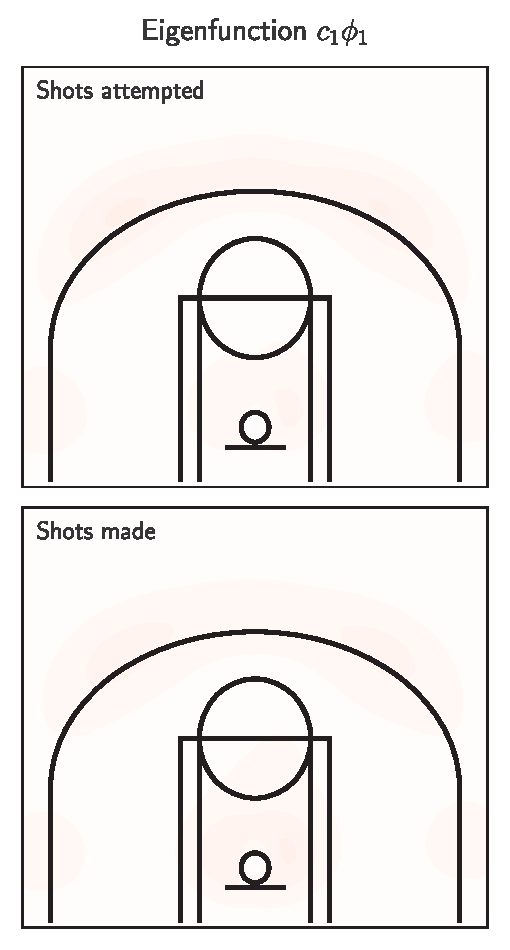
\includegraphics[scale=0.4]{figures/cluster_3_eigenfunction_1.eps}
%     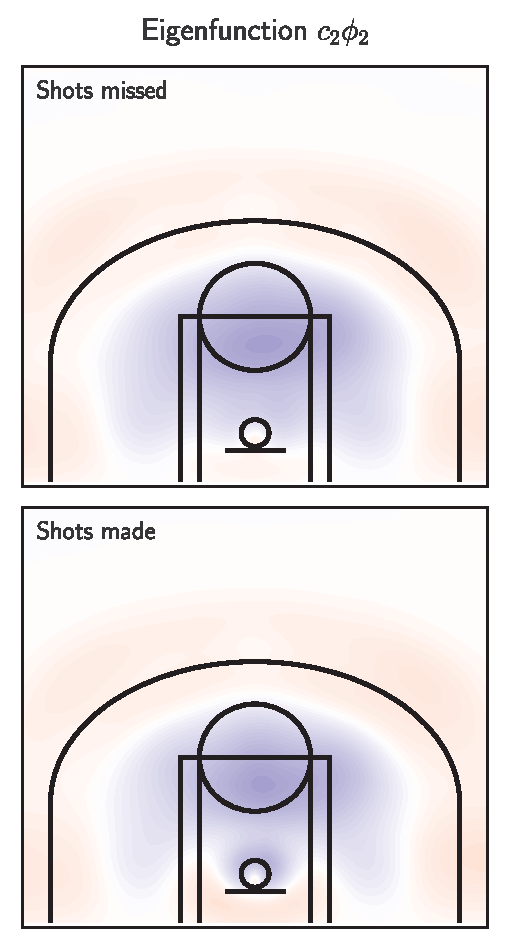
\includegraphics[scale=0.4]{figures/cluster_3_eigenfunction_2.eps}
%     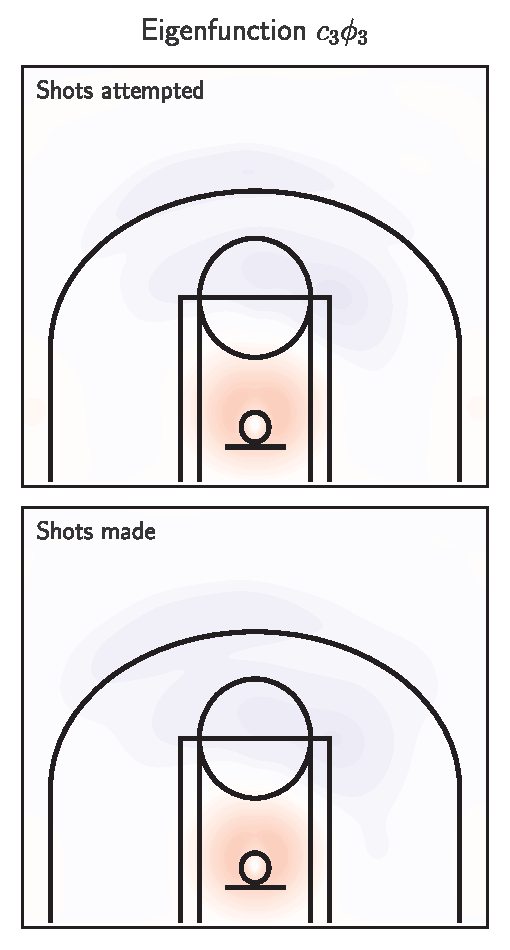
\includegraphics[scale=0.4]{figures/cluster_3_eigenfunction_3.eps}
%     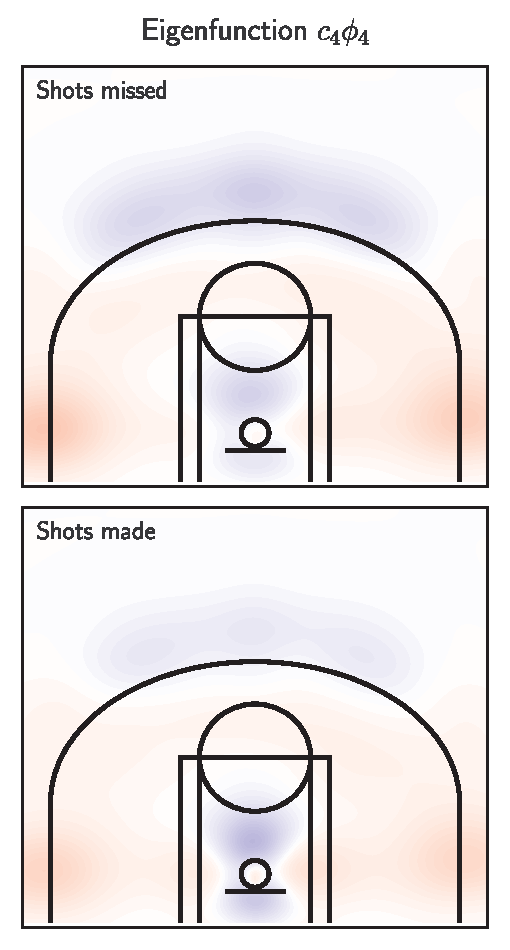
\includegraphics[scale=0.4]{figures/cluster_3_eigenfunction_4.eps}
%     \caption{Cluster 3}
%     \label{fig:clusters_3}
% \end{figure}

% From Figure~\ref{fig:clusters_4}, the average player in cluster $4$ shots more than the other player in the NBA (large positive coefficient). They prefer to shots 3-pointers than 2-pointers (negative coefficients for $\phi_2$ and $\phi_3$). They also prefer to shot in the corners (negative coefficients for $\phi_4$).
% \begin{figure}
%     \centering
%     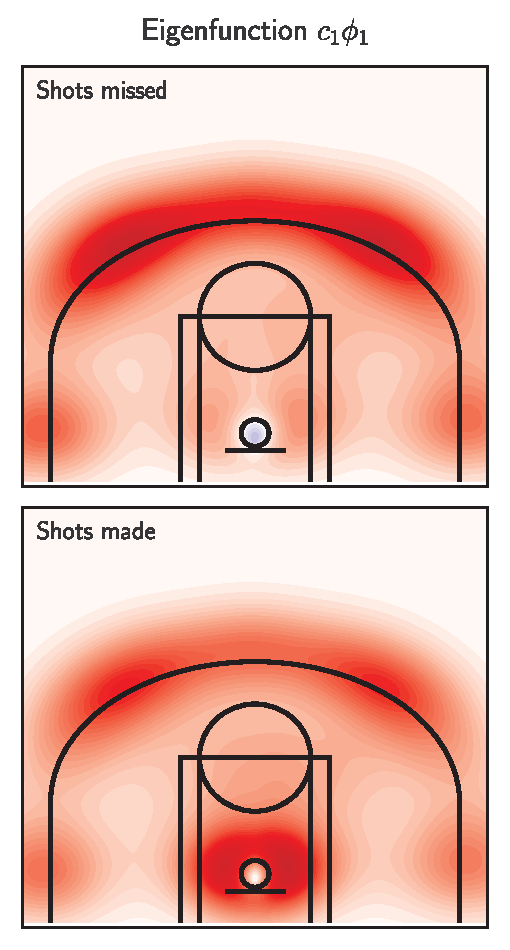
\includegraphics[scale=0.4]{figures/cluster_4_eigenfunction_1.eps}
%     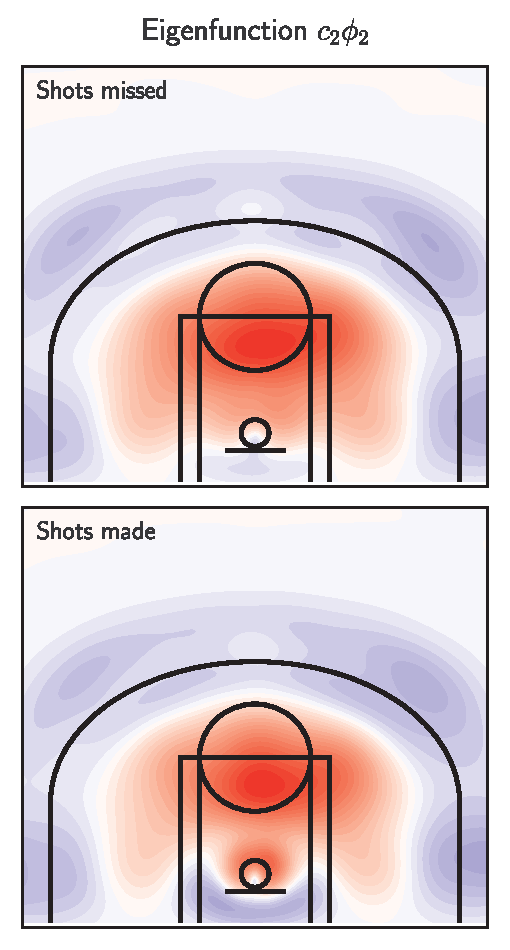
\includegraphics[scale=0.4]{figures/cluster_4_eigenfunction_2.eps}
%     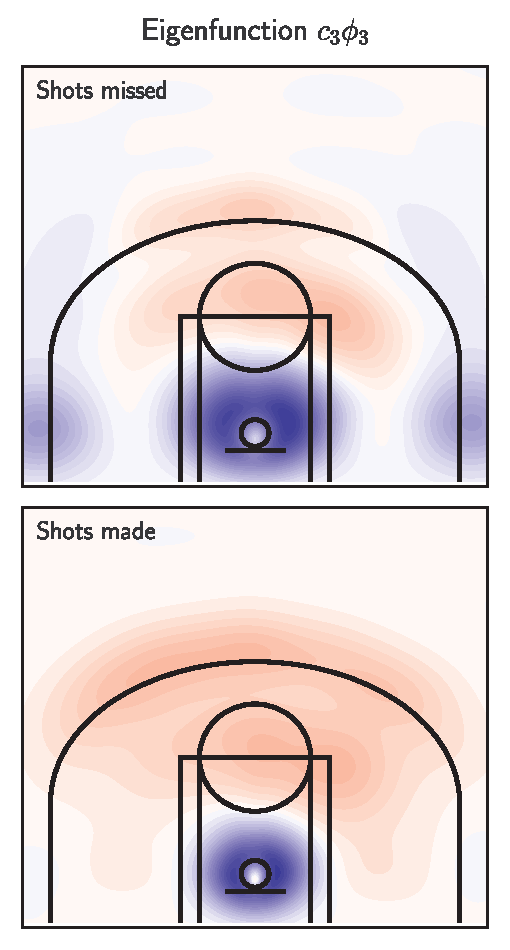
\includegraphics[scale=0.4]{figures/cluster_4_eigenfunction_3.eps}
%     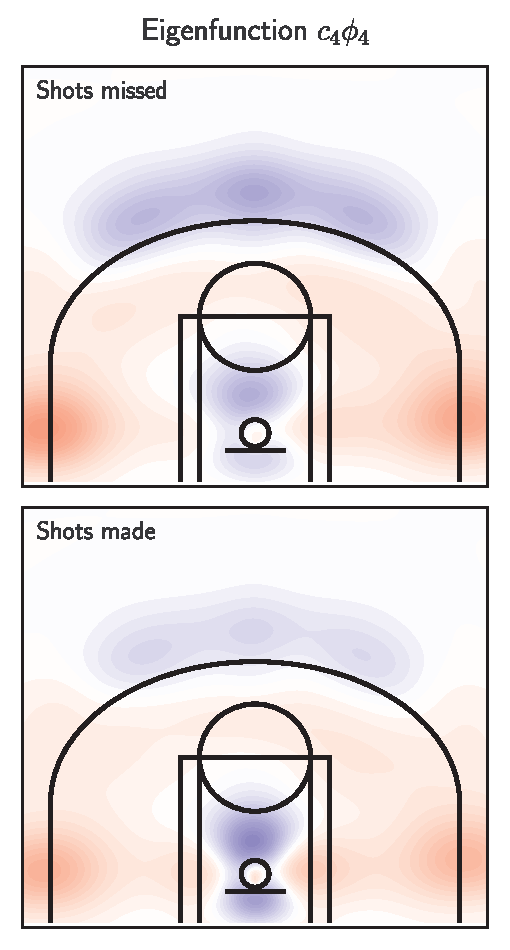
\includegraphics[scale=0.4]{figures/cluster_4_eigenfunction_4.eps}
%     \caption{Cluster 4}
%     \label{fig:clusters_4}
% \end{figure}

% Players from the last cluster (see Figure~\ref{fig:clusters_5}) shot less than  the average NBA player without any particular preference for any position.
% \begin{figure}
%     \centering
%     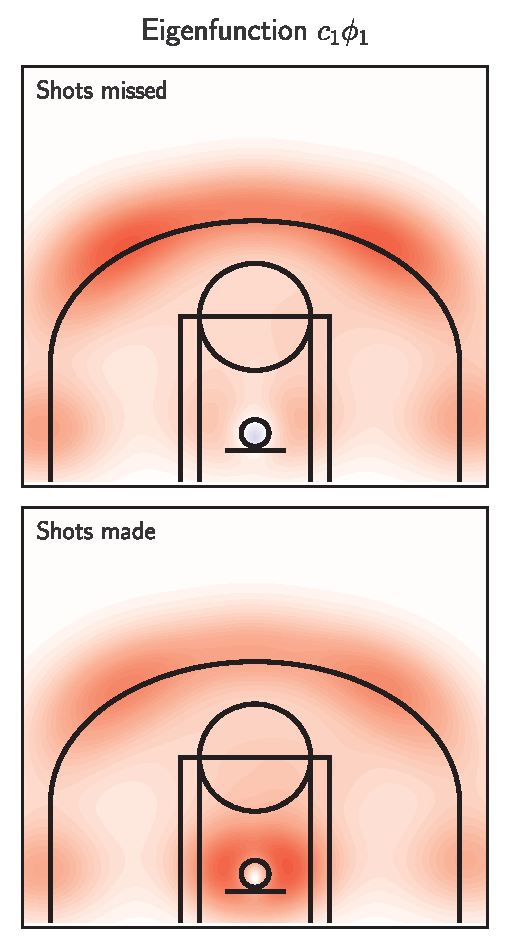
\includegraphics[scale=0.4]{figures/cluster_5_eigenfunction_1.eps}
%     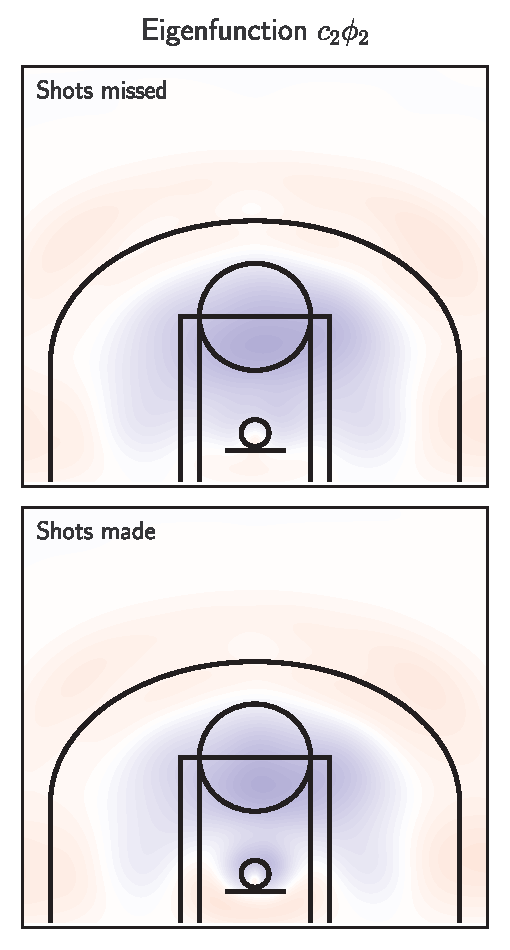
\includegraphics[scale=0.4]{figures/cluster_5_eigenfunction_2.eps}
%     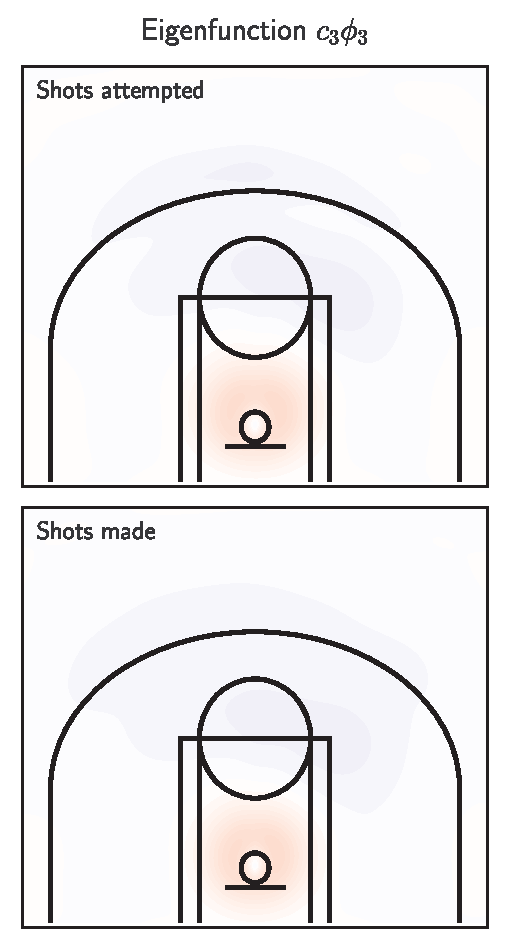
\includegraphics[scale=0.4]{figures/cluster_5_eigenfunction_3.eps}
%     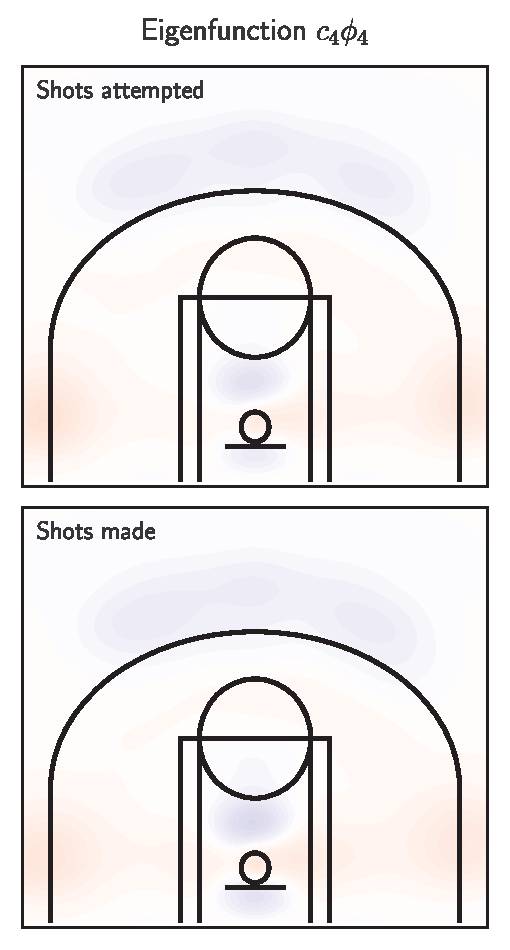
\includegraphics[scale=0.4]{figures/cluster_5_eigenfunction_4.eps}
%     \caption{Cluster 5}
%     \label{fig:clusters_5}
% \end{figure}

% subsection clustering (end)

% section results (end)